\documentclass{standalone}

\usepackage{tikz}

\begin{document}

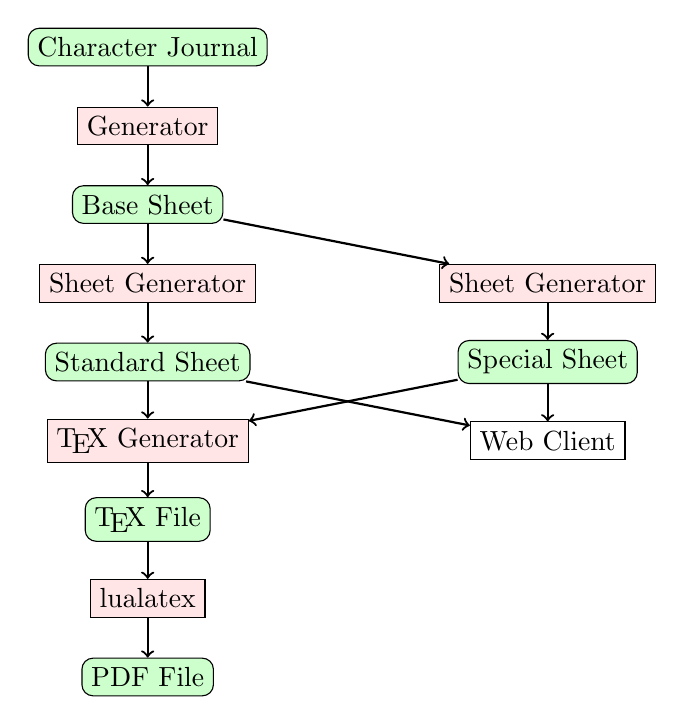
\begin{tikzpicture}
   \tikzstyle{file}=[fill=green!20,rounded corners,draw]
   \tikzstyle{transform}=[fill=red!10,draw]
   \tikzstyle{arrow}=[thick,draw,->]
   \node (cj) [file] {Character Journal} ;
   \node (gen) [transform,below of=cj] {Generator} ;
   \node (base) [file,below of=gen] {Base Sheet} ;
   \node (sgen) [transform,below of=base] {Sheet Generator} ;
   \node (sheet) [file,below of=sgen] {Standard Sheet} ;
   \node (sgen2) [transform,right of=sgen,node distance=2in] {Sheet Generator} ;
   \node (sheet2) [file,below of=sgen2] {Special Sheet} ;
   \path [arrow] (cj) -> (gen) ;
   \path [arrow] (gen) -> (base) ;
   \path [arrow] (base) -> (sgen) ;
   \path [arrow] (base) -> (sgen2) ;
   \path [arrow] (sgen) -> (sheet) ;
   \path [arrow] (sgen2) -> (sheet2) ;
   \node (tgen) [transform,below of=sheet] {\TeX\ Generator} ;
   \path [arrow] (sheet) -> (tgen) ;
   \path [arrow] (sheet2) -> (tgen) ;
   \node (tgen) [transform,below of=sheet] {\TeX\ Generator} ;
   \node (tex) [file,below of=tgen] {\TeX\ File} ;
   \node (luatex) [transform,below of=tex] {lualatex} ;
   \node (pdf) [file,below of=luatex] {PDF File} ;
   \path [arrow] (tgen) -- (tex) ;
   \path [arrow] (tex) -- (luatex) ;
   \path [arrow] (luatex) -- (pdf) ;
   \node (web) [draw,right of=tgen,node distance=2in] {Web Client} ;
   \path [arrow] (sheet) -> (web) ;
   \path [arrow] (sheet2) -> (web) ;
\end{tikzpicture}

\end{document}
